\section{Amélioration du prefetch de Blue Banana}

L'objectif  dt rapatrier plus finement les données que ce qui a pu être fait dans Blue Banana, et surtout d'essayer de ne pas rapatrier des données inutiles. Pour le moment, nous regardons juste les nœuds qui sont dans notre champs de vision (un cône) et qui ne sont ni trop loin, ni trop près. Mais il serait intéressant d'avoir plus d'informations sur les nœuds avant de les rapatrier, comme leur direction ou leur vitesse par exemple. Nous avons donc regarder quelques critères pourraient permettre de rapatrier les données plus intelligemment.

\subsection{Les changements introduits sur la version de Blue Banana}


\par Actuellement un nœud, qui est dans l'état \textbf{T}(ravelling), va chercher des nœuds qui se trouvent sur la trajectoire probable de l'avatar, tant que son ensemble de voisins n'est pas plein. Ce mécanisme va donc rapatrier des données qui sont à bonne distance (pas trop près à cause des temps de communication). Un des risques difficilement évitable est de rapatrier des nœuds qui sont inutiles si l'avatar, dont nous rapatrions les données, change de direction ou d'état. Un autre problème est que l'on peut rapatrier des avatars qui sont dans le cônes mais qui s'en écartent ou des avatars qui arrivent à grand vitesse vers notre avatar (voir figure~\ref{prefetchav}). Le mécanisme existant n'observent pas les différentes propriétés des nœuds (vitesse, direction, état, etc). Des nœuds surement superflu vont dans être rapatrier, modifier le prefetch pourrait nous permettre de de faire ce traitement plus finement.

\par  Nous pouvons voir un exemple de l'avantage de cet ajout (voir figure~\ref{prefetchav}), qui pourrait, par exemple, permettre l'ajout du nœud en rouge au lieu du vert.

	\begin{figure}[!h]
        \centering
        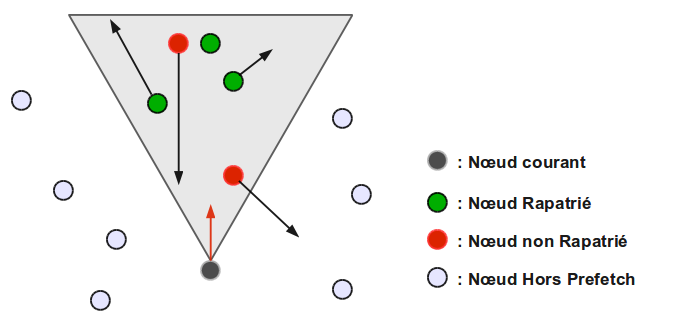
\includegraphics[scale=0.45]{./Ressources/Images/prefetchaV1.png}
        \caption{Exemple de gain possible pour le prefetching}
        \label{prefetchav}
        \end{figure}

\par L'idée est donc en plus de la distance avec le nœud de tester les différentes propriétés. Dans les messages actuelles, nous avons le vecteur du nœud de base. Nous pourrons, grâce à lui, regarder la direction et la longueur du nœud qui souhaite prefetcher et du nœud courant. Nous avons commencé par filtrer les nœuds qui étaient dans l'état \textbf{T}(ravelling), en faisant la somme du vecteur de prefetch et de celui du nœud courant ainsi si la norme est plus grande que la norme du prefetch, nous sélectionnons ce nœud et nous faisons le traitement correspondant. Cette solution laissant passer le problème de nœud qui arrive à grand vitesse vers le nœud ou qui s'en écartent, nous avons chercher à regarder les directions des différents nœud et de les comparer.
\par En utilisant les directions, une des idées a été de rapatrier de préférence les nœuds qui vont dans la même direction (vois figure~\ref{PrefetchSol}). Si les nœuds vont vers les cotés, par rapport au vecteur de prefetch, il faut que la longueur du vecteur soit alors pas trop grande pour qu'il soit rapatrier. De même pour le nœuds qui vont dans la direction opposés au vecteur de prefetch.

	\begin{figure}[!h]
        \centering
        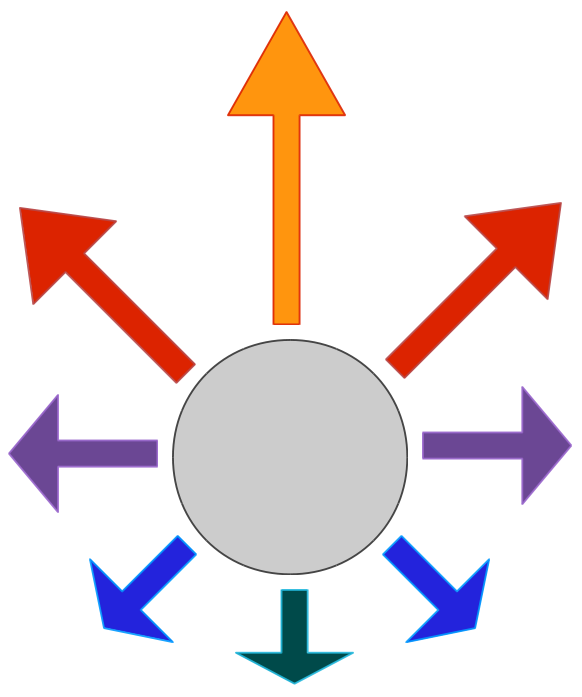
\includegraphics[scale=0.30]{./Ressources/Images/prefetchSol.png}
        \caption{Préférence de prefetching}
        \label{PrefetchSol}
        \end{figure}

\par Les ajouts ont été fait dans le module de mise en place du prefetch de Blue Banana. Des fonctions de comparaisons d'angle et de norme y ont été ajouté, et nous les avons insérer dans la fonction \textit{processPrefetchMsg} (voir figure~\ref{codePrefetch}). Après avoir fait les traitements de base, commme vérifier que le nœud soit assez loin, nous testons pour savoir si le prefetch amélioré est activé. 
\newline
\\ Dans ce cas, nous rapatrions si:
        \begin{itemize}
        \renewcommand{\labelitemi}{$\bullet$}
                \item L'angle du vecteur du nœud courant est proche de l'angle du vecteur de prefetch (environ 45° de chaque côté).
		\item La somme des normes est supérieur à celle du vecteur de prefetch multilié par un et demi. 
                \item Le nœud courant n'est pas dans l'état \textbf{T}(ravelling).
		\item L'angle du vecteur du nœud courant n'est pas proche de l'angle du vecteur du nœud de prefetch mais la norme du nœud courant est inférieur à celle du nœud de prefecth. 
        \end{itemize}


\lstset{numbers=left,basicstyle=\scriptsize, numberstyle=\tiny, stepnumber=5, numbersep=5pt}

\lstinputlisting[title={\underline{\textbf{Partie du code de la fonction processPrefetchMsg}}},label={codePrefetch}]{./Ressources/Documents/ProcessPrefetchMsg.java}


\subsection{Les résultats et les observations sur le prefetch amélioré}



\subsection{Conclusion et perspectives}
Mieux regarder les directions, en fonction de la distance des nœuds avec le nœud qui souhaite rapatrier, pourrait peut être permettre de mieux choisir les nœuds.
Une autre amélioration pourrait être de chercher parmi des nœuds qui peuvent être hors du cône, mais sans aller trop loin pour ne pas rajouter trop de nœuds à contacter sinon trop de messages seraient alors émis. Si ce mécanisme permet de d'augmenter l'efficacité du prefetch, il peut aussi être possible de regarder avec un angle plus grand de façon périodique.


\newpage
